\documentclass[10pt]{beamer}

\usetheme{metropolis}
\usepackage{appendixnumberbeamer}

\usepackage{booktabs}
\usepackage[scale=2]{ccicons}

\usepackage{pgfplots}
\usepgfplotslibrary{dateplot}

\usepackage{xspace}
\newcommand{\themename}{\textbf{\textsc{metropolis}}\xspace}
\usepackage{tabularx}

\usepackage[utf8]{inputenc}
\usepackage[brazilian]{babel}

\title{Mudança de Conceito}
\subtitle{Definição, técnicas e ferramentas}
\date{}
\author{Ruivaldo Neto}
\institute{UFBA - PGCOMP}
\titlegraphic{\hfill
\includegraphics[scale=0.43]{logo.png}}

\begin{document}

\maketitle

\begin{frame}{Roteiro}
  \setbeamertemplate{section in toc}[sections numbered]
  \begin{minipage}{\textwidth}
    \tableofcontents
  \end{minipage}
\end{frame}

\section{Introdução}

\begin{frame}{Introdução}
    Algoritmos de aprendizagem não melhoram pelo simples passar do tempo.

    \begin{figure}[H]
        \begin{center}
            
\includegraphics[scale=0.8]{wine.png}
        \end{center}
    \end{figure}
\end{frame}

\begin{frame}{Introdução}
    Parte significativa das técnicas foi projetada para cenários \textbf{estacionários}, 
    onde se assume que: 
    
    \texttt{distribuição de treinamento} $=$ \texttt{distribuição de operação}.

    \begin{figure}[H]
        \begin{center}
            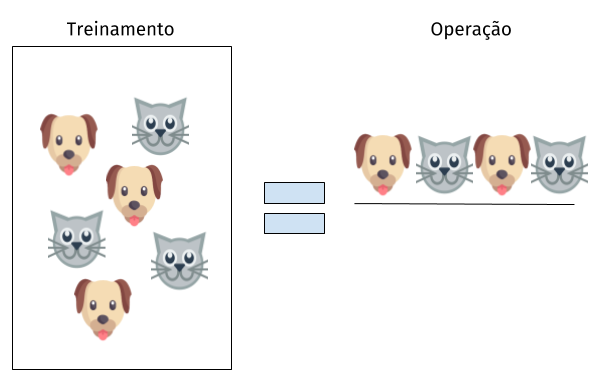
\includegraphics[scale=0.5]{treinamento_operacao_estacionario.png}
        \end{center}
    \end{figure}
\end{frame}

\begin{frame}{Introdução}
    As aplicações reais são, em sua maioria, \textbf{não-estacionárias}, isto é:

    \texttt{distribuição de treinamento} $\neq$ \texttt{distribuição de operação}.

    \begin{figure}[H]
        \begin{center}
            
\includegraphics[scale=0.45]{mudanca_populacao_conceitos_emergentes.png}
        \end{center}
    \end{figure}
\end{frame}

\begin{frame}{Introdução}
    Uma solução comum, mas \textbf{pobre}, é a execução de treinamentos recorrentes.

    \begin{figure}[H]
        \begin{center}
            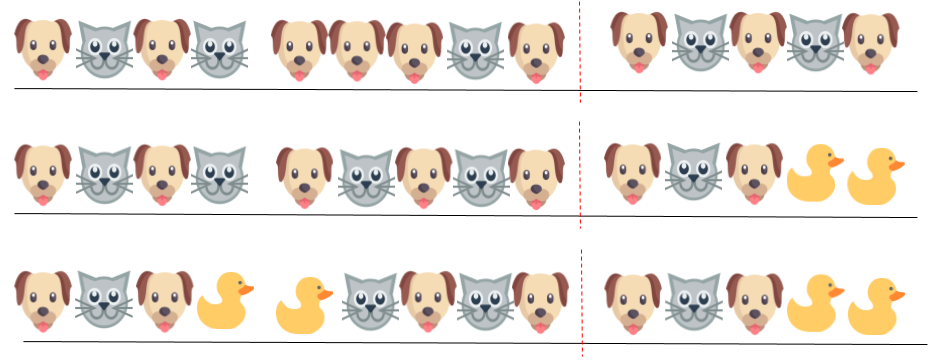
\includegraphics[scale=0.45]{treinamentos_recorrentes.png}
        \end{center}
    \end{figure}
\end{frame}

\begin{frame}{Introdução}
    Técnicas de aprendizado ativo diminuem o custo de rotulação, mas não são capazes de lidar com mudanças de conceito.

    \begin{figure}[H]
        \begin{center}
            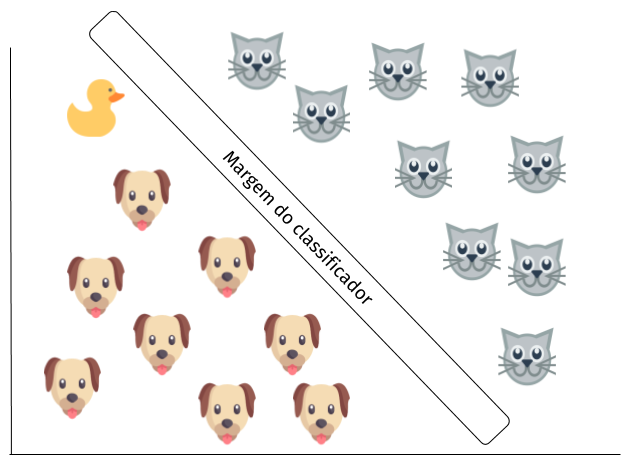
\includegraphics[scale=0.45]{active_learning.png}
        \end{center}
    \end{figure}
\end{frame}

\begin{frame}{Introdução}
    Solução: \textbf{monitoramento}.
    
    \begin{figure}[H]
        \begin{center}
            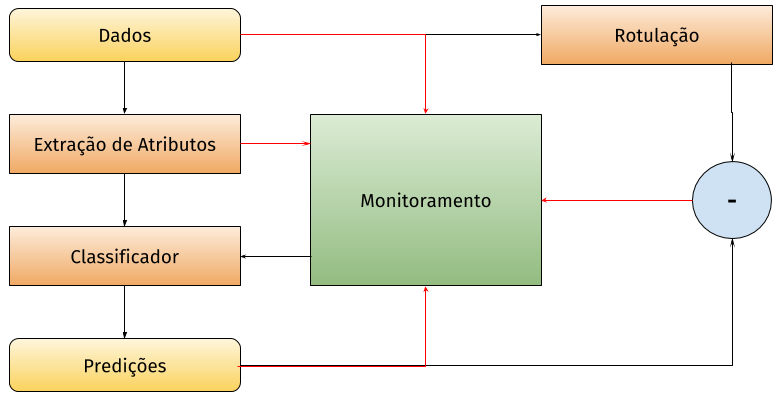
\includegraphics[scale=0.45]{solucao_melhor.png}
        \end{center}
    \end{figure}
\end{frame}

\section{Formalização}

\begin{frame}{Formalização}
    A Teoria Bayesiana é comumente aplicada para descrever as tarefas de classificação \cite{Duda:2000:PC:954544}.
    A partir dela, também é possível formalizar o problema de mudança de conceito.
\end{frame}


\begin{frame}{Formalização}
    Considerando $X \in \mathbb{R}^p$ uma instância em um espaço $p$-dimensional de atributos e $X \in c_i$ onde $c_1$, $c_2$, \ldots, $c_k$ é o conjunto de classes, 
    o classificador ótimo para classificar $x \rightarrow c_i$ é determinado pelas probabilidades a priori das classes, $P(c_i)$, e a função de densidade de probabilidade condicionada às classes, $p(X|c_i)$, para $i = 1, \ldots, k$.
\end{frame}

\begin{frame}{Formalização}
Dessa forma, um conceito pode ser definido como um conjunto de probabilidades a priori e condicionais das classes (Eq. \ref{eq:conceito}):

\begin{equation} \label{eq:conceito}
    S = \{(P(c_1), P(X|c_1)), (P(c_2), P(X|c_2)), ..., (P(c_k), P(X|c_k))\}
\end{equation}
\end{frame}

\begin{frame}{Formalização}
Ainda segundo a Teoria Bayesiana, a classificação baseada na máxima probabilidade a posteriori de uma instância $X$ pode ser obtida através da Equação \ref{eq:classificacao}:

\begin{equation} \label{eq:classificacao}
    p(c_i|X) = \frac{p(c_i) * p(X|c_i)}{p(X)}
\end{equation}
\end{frame}

\begin{frame}{Formalização}
Sendo possível definir formalmente que há mudança de conceito entre os instantes $t_0$ e $t_1$ se:

\begin{equation} \label{eq:3}
    {\exists}X : p_{t_0}(X, c) \ne p_{t_1}(X, c)
\end{equation}

onde, $p_{t_0}$ e $p_{t_1}$ denotam as distribuições de probabilidades conjuntas nos instantes $t_0$ e $t_1$, respectivamente, 
para $X$ e $c$ \cite{Gama:2014:SCD:2597757.2523813}. 
\end{frame}

\begin{frame}{Formalização}
Com base na formalização exposta \cite{Zliobaite:2010}, pode-se definir que mudanças de conceito ocorrem devido a:

\begin{enumerate}
    \item Alterações na probabilidade a priori das classes $P(c)$;
    \item Alterações na distribuição de uma ou mais classes $p(X|c)$;
    \item Alterações nas distribuições a posteriori das classes $p(c|X)$.
\end{enumerate}
\end{frame}

\section{Tipos, Padrões e Taxonomia}

\begin{frame}{Tipos}
    \begin{itemize}
        \item \textbf{Virtuais:} indicam mudanças na probabilidade a priori das classes, $P(c)$, e não têm impacto nos conceitos-alvo.
        \item \textbf{Reais:} referem-se a mudanças na probabilidade a posteriori, $p(c|X)$, e afetam os conceitos-alvo.
    \end{itemize} 

    \begin{figure}[H]
    \begin{center}
        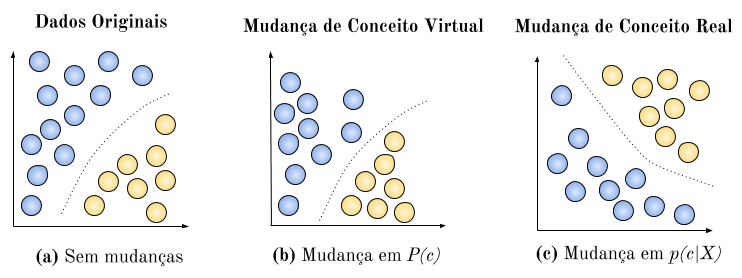
\includegraphics[scale=0.5]{imagens/concept_drift.png}
    \end{center}
    \end{figure}
\end{frame}
 
\begin{frame}{Padrões}
    As mudanças de conceito podem ocorrer de forma abrupta, gradual, incremental ou recorrente \cite{Gama:2014:SCD:2597757.2523813}:

    \begin{figure}[H]
    \begin{center}
        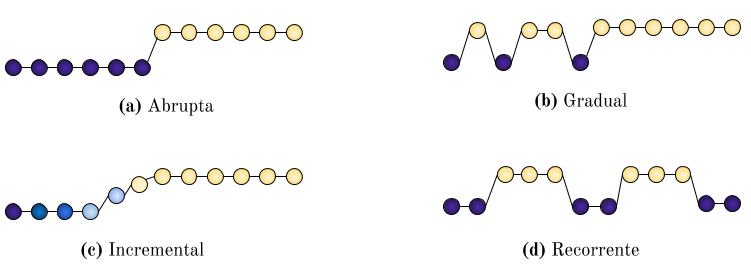
\includegraphics[scale=0.5]{imagens/concept_drift_patterns.png}
    \end{center}
    \end{figure}
\end{frame}

\begin{frame}{Taxonomia}
    Termos correspondentes a \textbf{mudança de conceito} em cada área de pesquisa \cite{Zliobaite:2010}:

    \begin{center} 
    \begin{table}[H]
    \label{tbl:taxonomy}
    \begin{tabularx}{\textwidth}{|l|X|}
    \cline{1-2}
    \multicolumn{1}{|c|}{\textbf{Área}} & \multicolumn{1}{c|}{\textbf{Termos}}       \\ \cline{1-2}
    Mineração de Dados                  & Mudança de Conceito                        \\ \cline{1-2}
    Aprendizado de Máquina              & Mudança de Conceito, Mudança de Covariável \\ \cline{1-2}
    Computação Evolucionária            & Ambiente Evolutivo, Ambiente em Mudança    \\ \cline{1-2}
    IA e Robótica                       & Ambiente Dinâmico                          \\ \cline{1-2}
    Estatísticas, Séries Temporais      & Não Estacionário                           \\ \cline{1-2}
    Recuperação de Informação           & Evolução Temporal                          \\ \cline{1-2}
    \end{tabularx}
    
    \end{table}
    \end{center}
\end{frame}

\begin{frame}{Taxonomia}
    Os termos Detecção de \textit{Outliers}, Detecção de Novidade, Detecção de \textit{Change Points} e Detecção de Mudança de Conceito, apesar de próximos, possuem significados diferentes:

    \begin{itemize}
        \item \textbf{Detecção de \textit{Outliers}}: identificam padrões em desacordo com o comportamento esperado \cite{Chandola:2009:ADS:1541880.1541882}.
        \item \textbf{Detecção de Novidade}: identificam padrões ainda não observados e incorporam ao modelo \cite{Chandola:2009:ADS:1541880.1541882}.
        \item \textbf{Detecção de \textit{Change Points}}: identificam variações abruptas de valor, que podem representar transições entre estados, em séries temporais unidimensionais estacionárias \cite{Aminikhanghahi:2017:SMT:3086013.3086037}.
    \end{itemize}
\end{frame}

\section{Técnicas de detecção}

\begin{frame}{Técnicas de detecção - Categorias}
    \begin{itemize}
        \item \textbf{Algoritmos Explícitos/Supervisionados}: Dependem da rotulação dos dados, pois são utilizados no cálculo das medidas de performance.
        \item \textbf{Algoritmos Implícitos/Não Supervisionados}: Independem de rotulação. Baseiam-se nas características dos dados. 
    \end{itemize}
\end{frame}

\begin{frame}{Técnicas de detecção - Supervisionados}
    Os algoritmos supervisionados dividem-se em três grupos principais \cite{Gama:2014:SCD:2597757.2523813}:

    \begin{itemize}
        \item \textbf{Métodos Baseados em Análise Sequencial}: Monitoram os resultados das predições (taxa de erro).
        \item \textbf{Abordagens baseadas em Estatística}: Monitoram os resultados das predições conforme parâmetros estatísticos (média, desvio padrão, etc).
        \item \textbf{Métodos baseados em Janelas}: Mantém o sumário da distribuição de uma janela passada como treinamento. Comparam este sumário com a distribuição da janela atual.
    \end{itemize}
\end{frame}

\begin{frame}{Técnicas de detecção - Não Supervisionados}
    Os algoritmos não supervisionados também foram divididos em três grupos \cite{GONCALVES20148144}:

    \begin{itemize}
        \item \textbf{Detecção de Novidade / Métodos de Agrupamento}: Utilizam a distância e/ou a densidade dos dados para detectar novos padrões.
        \item \textbf{Monitoramento de distribuição multivariada}: Monitoram diretamente a distribuição dos dados, considerando seus atributos.
        \item \textbf{Monitoramento dependente de modelo}: Restringem-se aos classificadores probabilísticos, pois monitoram as probabilidades a posteriori.
    \end{itemize}
\end{frame}

\begin{frame}{Técnicas de detecção - Resumo}
    Resumo das categorias, grupos e técnicas:

    % Please add the following required packages to your document preamble:
    % \usepackage{graphicx}
    \begin{table}[!ht]
        \centering
        \resizebox{\textwidth}{!}{%
        \begin{tabular}[t]{@{}lllll@{}}
        \hline \\
        Algoritmos Explícitos/Supervisionados     & Métodos Baseados em Análise Sequencial        & \begin{tabular}[t]{@{}l@{}} Cumulative Sum (CUSUM) \\ PageHinkley (PH) \cite{Page:CUSUM:PageHinkley:1954} \\ Geometric Moving Average (GMA) \cite{Roberts:2000:CCT:338441.338464}\end{tabular}                                                                                                                        &  &  \\ \\
                                                & Abordagens baseadas em Estatística            & \begin{tabular}[t]{@{}l@{}} Drift Detection Method (DDM) \cite{GamaMCR04} \\  Early Drift Detection Method (EDDM) \cite{EDDM} \\  Exponentially Weighted Moving Average (EWMA) \cite{Ross:2012:EWM:2076039.2076307} \\ Reactive Drift Detection Method (RDDM) \cite{Barros:RDDM:2017} \end{tabular}                                                                &  &  \\ \\
                                                & Métodos baseados em Janelas                   & \begin{tabular}[t]{@{}l@{}} Adaptive Windowing (ADWIN) \cite{BifetG07} \\   SeqDrift \cite{PearsSK14:SeqDrift:2014} \\   HDDMA/HDDMW \cite{BlancoCRBDM15:HDDMA:HDDMW:2015} \end{tabular}                                                                                            &  &  \\ \\
        
        Algoritmos Implícitos/Não Supervisionados & Detecção de Novidade / Métodos de Agrupamento & \begin{tabular}[t]{@{}l@{}} OLINDDA \cite{Spinosa:2007:OCA:1244002.1244107} \\   MINAS \cite{Faria:2013:NDA:2480362.2480515} \\   Woo \cite{Ryu:Kantardzic:2012} \\   DETECTNOD \cite{Hashemi:Hayat:DETECTNOD:2010} \\   ECSMiner \cite{Masud:2011:CNC:1978259.1978529} \\   GC3 \cite{Sethi2016b:GC3} \end{tabular} &  &  \\ \\
                                                & Monitoramento de distribuição multivariada    & \begin{tabular}[t]{@{}l@{}} CoC \cite{Lee:Magoules:CoC:2012} \\ HDDDM \cite{Ditzler:Polikar:HDDDM:2011} \\ PCA-detect \cite{Kuncheva:PCADetect:20085} \end{tabular}                                       &  &  \\ \\
                                                & Monitoramento dependente de modelo            & \begin{tabular}[t]{@{}l@{}} A-distance \cite{Dredze:ADistance:2010585} \\ CDBD \cite{Lindstrom:CDBD:2013} \\ Margin \cite{Dries:Margin:2009} \end{tabular}                                                                                        &  &  \\ \\
        \hline
        \end{tabular}%
        }
    \end{table}
\end{frame}

\section{Ferramentas}

\begin{frame}{MOA – Massive Online Analysis}
    \begin{itemize}
        \item Principal framework para mineração de dados em fluxos contínuos.
        \item Código-aberto\footnote{https://github.com/Waikato/moa} e multi-plataforma (Java).
        \item Grande base de algoritmos e integração com o WEKA \cite{Hall:2009:WDM:1656274.1656278}.
        \item Ferramentas para avaliação de desempenho desses algoritmos.
    \end{itemize}

    \begin{figure}[H]
        \begin{center}
            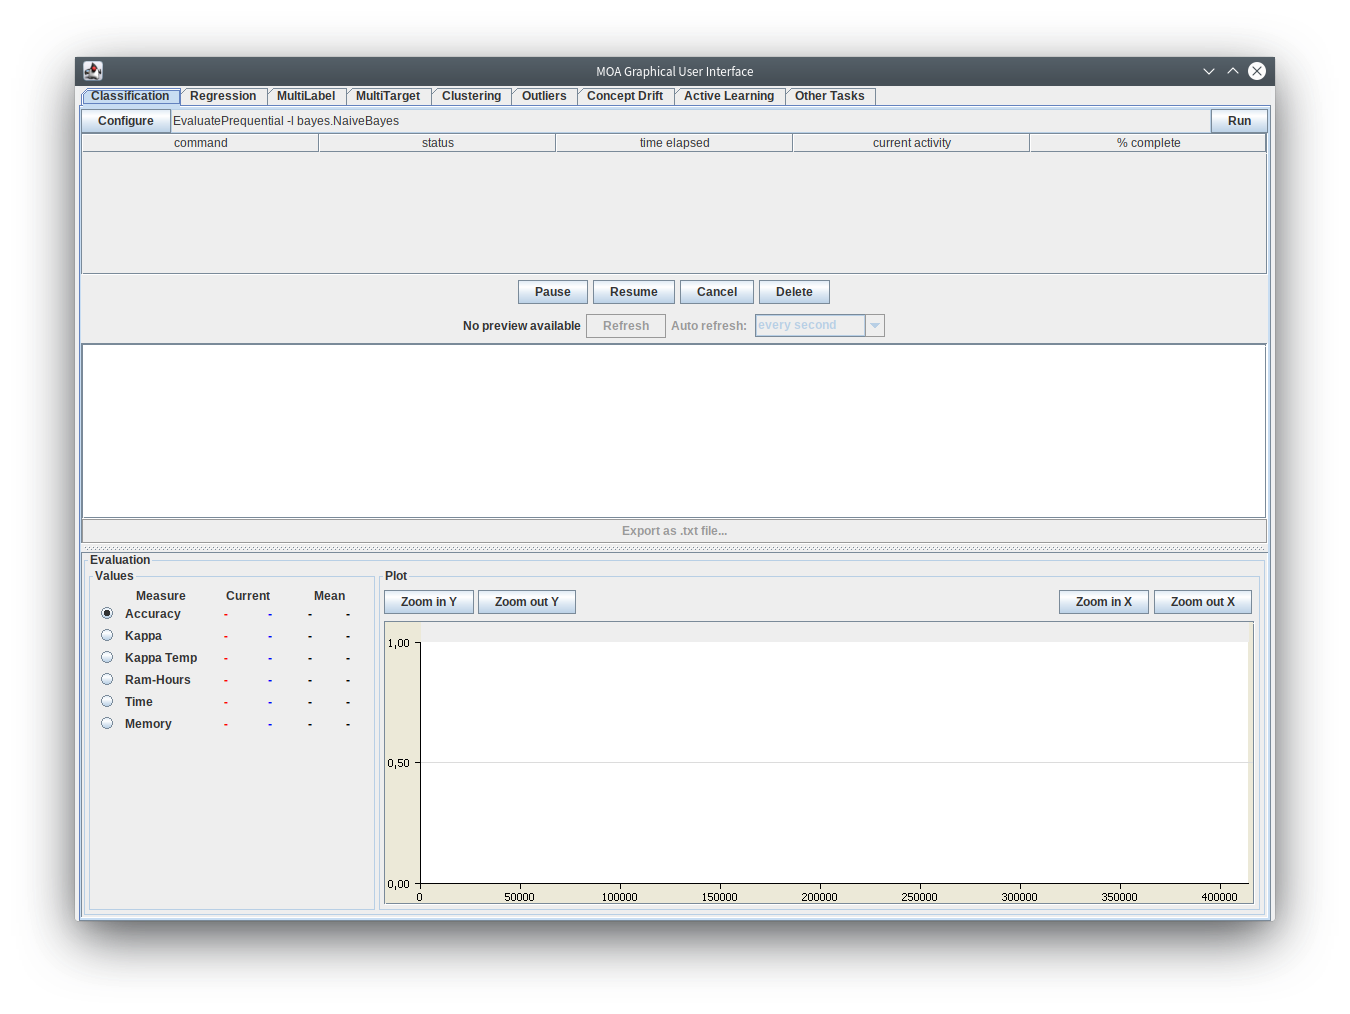
\includegraphics[scale=0.2]{imagens/moa.png}
        \end{center}
    \end{figure}
\end{frame}

\begin{frame}{MOA - Massive Online Analysis}
    \begin{itemize}
        \item Novos detectores de mudança de conceito podem ser criados estendo a classe abstrata \texttt{AbstractChangeDetector}.
        \item Interface de configuração é criada dinamicamente, a partir dos atributos da classe.
    \end{itemize}

    \begin{figure}[H]
        \begin{center}
            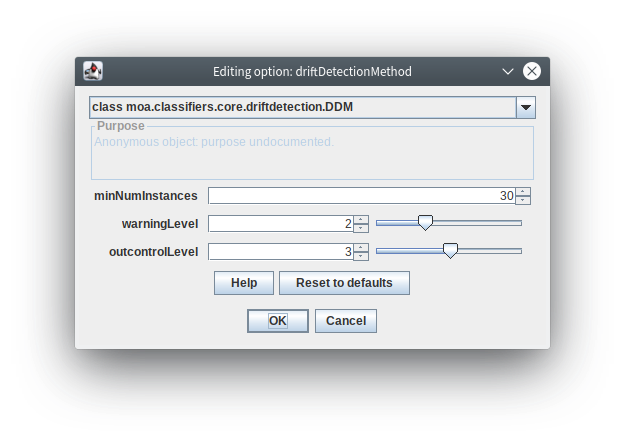
\includegraphics[scale=0.5]{imagens/detector.png}
        \end{center}
    \end{figure}
\end{frame}

\begin{frame}{MOA - Massive Online Analysis}
    \begin{itemize}
        \item Algoritmos para detecção de mudança de conceito podem ser avaliados pelos métodos \texttt{DriftDetectionMethodClassifier} ou \texttt{BasicConceptDriftPerformanceEvaluator}.
    \end{itemize}

    \begin{figure}[H]
        \begin{center}
            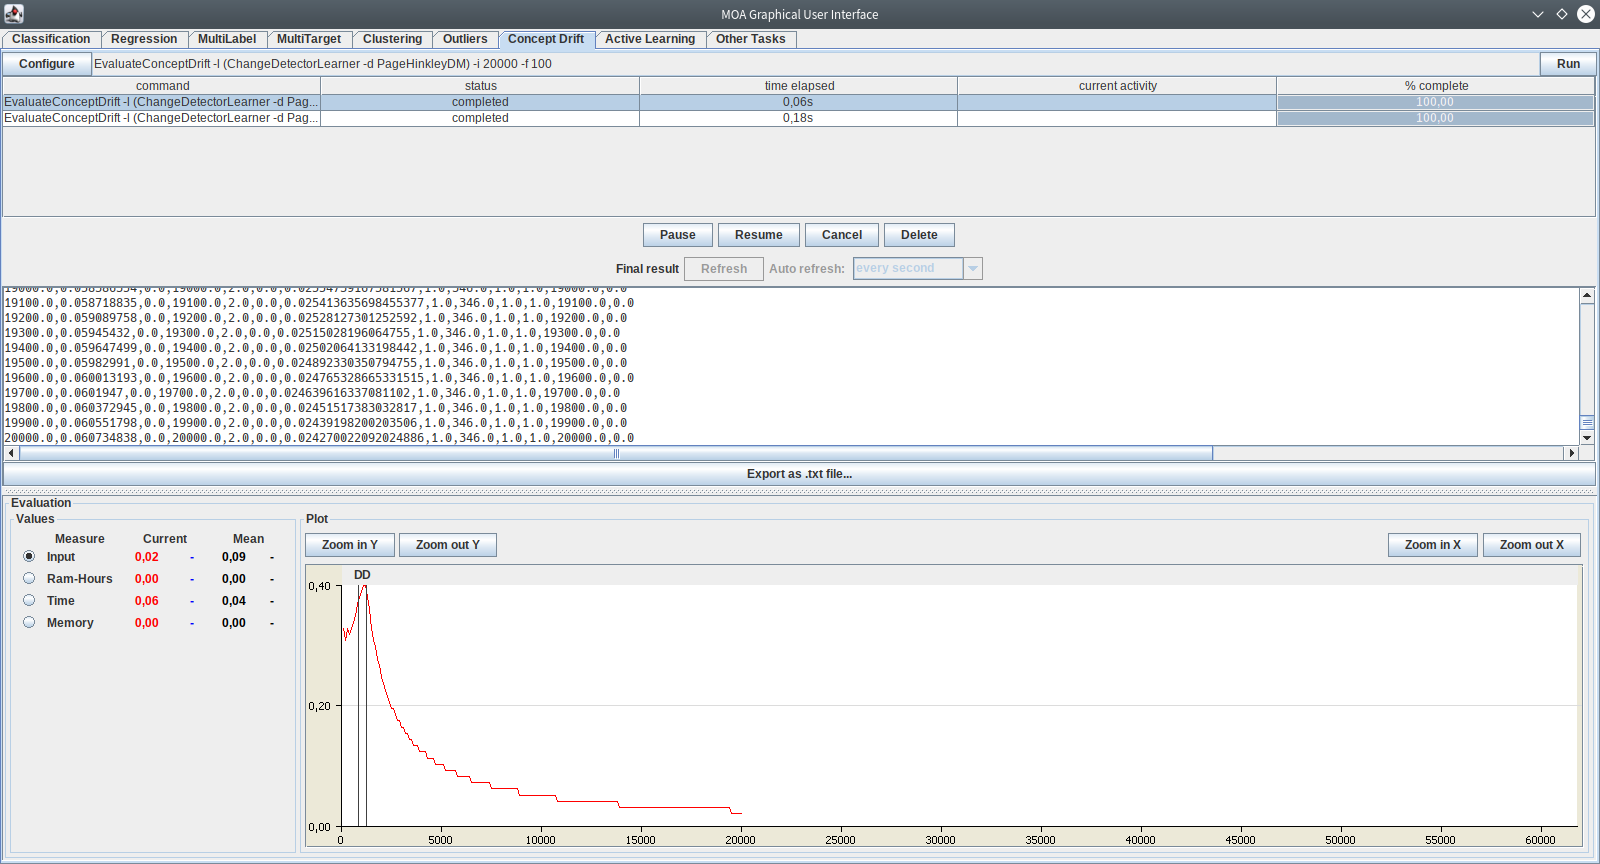
\includegraphics[scale=0.25]{imagens/moa_avaliacao_cd.png}
        \end{center}
    \end{figure}
\end{frame}

\begin{frame}{Tornado}
    \begin{itemize}
        \item Framework para avaliação de pares (classificador, detector de mudança de conceito) ao longo do tempo \cite{Pesaranghader:Tornado}.
        \item Código-aberto\footnote{https://github.com/alipsgh/tornado} e multi-plataforma (Python).
        \item Grande base de algoritmos implementados.
    \end{itemize}

    \begin{figure}[H]
        \begin{center}
            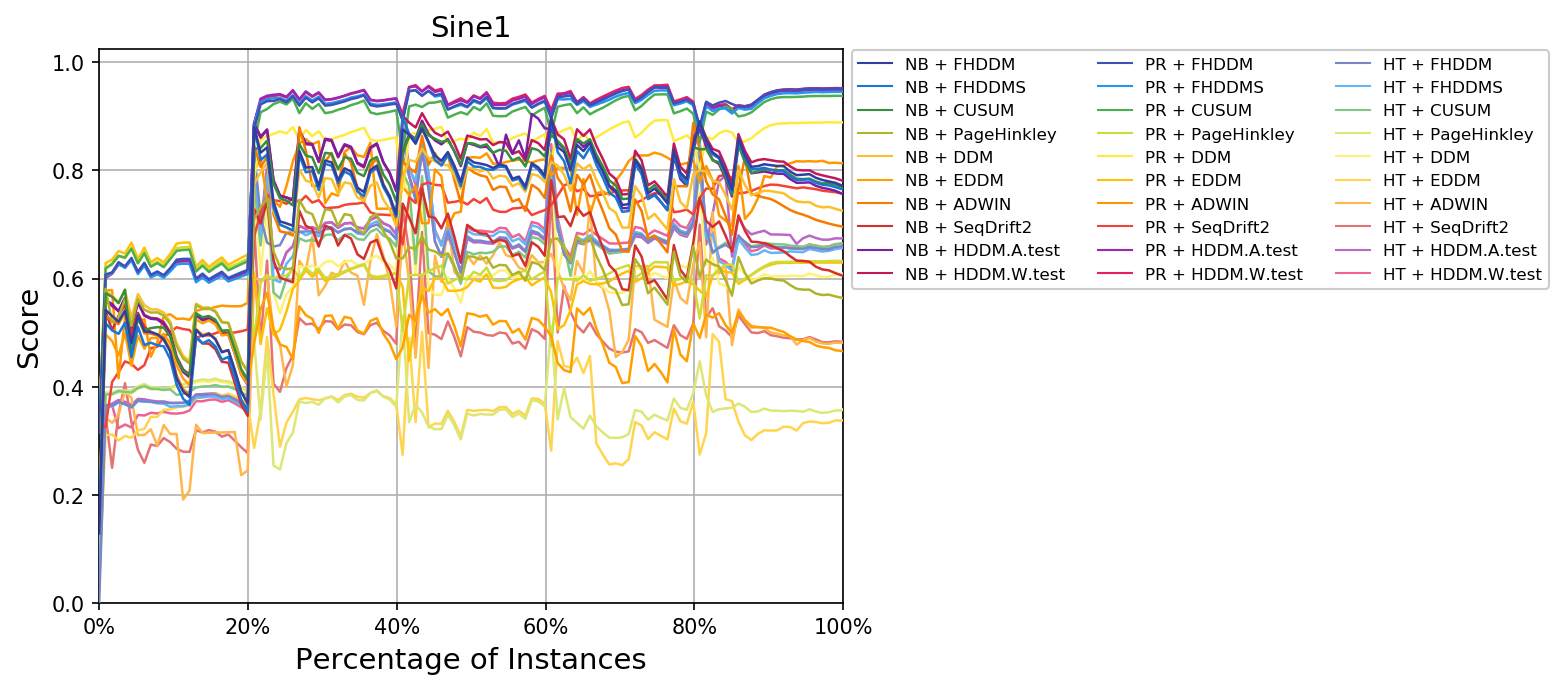
\includegraphics[scale=0.4]{imagens/tornado_out2.png}
        \end{center}
    \end{figure}
\end{frame}

\section{Conclusão}

\begin{frame}[standout]
  Obrigado! Dúvidas ?
\end{frame}

% \begin{frame}[fragile]{Metropolis}

%   The \themename theme is a Beamer theme with minimal visual noise
%   inspired by the \href{https://github.com/hsrmbeamertheme/hsrmbeamertheme}{\textsc{hsrm} Beamer
%   Theme} by Benjamin Weiss.

%   Enable the theme by loading

%   \begin{verbatim}    \documentclass{beamer}
%     \usetheme{metropolis}\end{verbatim}

%   Note, that you have to have Mozilla's \emph{Fira Sans} font and XeTeX
%   installed to enjoy this wonderful typography.
% \end{frame}
% \begin{frame}[fragile]{Sections}
%   Sections group slides of the same topic

%   \begin{verbatim}    \section{Elements}\end{verbatim}

%   for which \themename provides a nice progress indicator \ldots
% \end{frame}

% \section{Titleformats}

% \begin{frame}{Metropolis titleformats}
% 	\themename supports 4 different titleformats:
% 	\begin{itemize}
% 		\item Regular
% 		\item \textsc{Smallcaps}
% 		\item \textsc{allsmallcaps}
% 		\item ALLCAPS
% 	\end{itemize}
% 	They can either be set at once for every title type or individually.
% \end{frame}

% {
%     \metroset{titleformat frame=smallcaps}
% \begin{frame}{Small caps}
% 	This frame uses the \texttt{smallcaps} titleformat.

% 	\begin{alertblock}{Potential Problems}
% 		Be aware, that not every font supports small caps. If for example you typeset your presentation with pdfTeX and the Computer Modern Sans Serif font, every text in smallcaps will be typeset with the Computer Modern Serif font instead.
% 	\end{alertblock}
% \end{frame}
% }

% {
% \metroset{titleformat frame=allsmallcaps}
% \begin{frame}{All small caps}
% 	This frame uses the \texttt{allsmallcaps} titleformat.

% 	\begin{alertblock}{Potential problems}
% 		As this titleformat also uses smallcaps you face the same problems as with the \texttt{smallcaps} titleformat. Additionally this format can cause some other problems. Please refer to the documentation if you consider using it.

% 		As a rule of thumb: Just use it for plaintext-only titles.
% 	\end{alertblock}
% \end{frame}
% }

% {
% \metroset{titleformat frame=allcaps}
% \begin{frame}{All caps}
% 	This frame uses the \texttt{allcaps} titleformat.

% 	\begin{alertblock}{Potential Problems}
% 		This titleformat is not as problematic as the \texttt{allsmallcaps} format, but basically suffers from the same deficiencies. So please have a look at the documentation if you want to use it.
% 	\end{alertblock}
% \end{frame}
% }

% \section{Elements}

% \begin{frame}[fragile]{Typography}
%       \begin{verbatim}The theme provides sensible defaults to
% \emph{emphasize} text, \alert{accent} parts
% or show \textbf{bold} results.\end{verbatim}

%   \begin{center}becomes\end{center}

%   The theme provides sensible defaults to \emph{emphasize} text,
%   \alert{accent} parts or show \textbf{bold} results.
% \end{frame}

% \begin{frame}{Font feature test}
%   \begin{itemize}
%     \item Regular
%     \item \textit{Italic}
%     \item \textsc{SmallCaps}
%     \item \textbf{Bold}
%     \item \textbf{\textit{Bold Italic}}
%     \item \textbf{\textsc{Bold SmallCaps}}
%     \item \texttt{Monospace}
%     \item \texttt{\textit{Monospace Italic}}
%     \item \texttt{\textbf{Monospace Bold}}
%     \item \texttt{\textbf{\textit{Monospace Bold Italic}}}
%   \end{itemize}
% \end{frame}

% \begin{frame}{Lists}
%   \begin{columns}[T,onlytextwidth]
%     \column{0.33\textwidth}
%       Items
%       \begin{itemize}
%         \item Milk \item Eggs \item Potatos
%       \end{itemize}

%     \column{0.33\textwidth}
%       Enumerations
%       \begin{enumerate}
%         \item First, \item Second and \item Last.
%       \end{enumerate}

%     \column{0.33\textwidth}
%       Descriptions
%       \begin{description}
%         \item[PowerPoint] Meeh. \item[Beamer] Yeeeha.
%       \end{description}
%   \end{columns}
% \end{frame}
% \begin{frame}{Animation}
%   \begin{itemize}[<+- | alert@+>]
%     \item \alert<4>{This is\only<4>{ really} important}
%     \item Now this
%     \item And now this
%   \end{itemize}
% \end{frame}
% \begin{frame}{Figures}
%   \begin{figure}
%     \newcounter{density}
%     \setcounter{density}{20}
%     \begin{tikzpicture}
%       \def\couleur{alerted text.fg}
%       \path[coordinate] (0,0)  coordinate(A)
%                   ++( 90:5cm) coordinate(B)
%                   ++(0:5cm) coordinate(C)
%                   ++(-90:5cm) coordinate(D);
%       \draw[fill=\couleur!\thedensity] (A) -- (B) -- (C) --(D) -- cycle;
%       \foreach \x in {1,...,40}{%
%           \pgfmathsetcounter{density}{\thedensity+20}
%           \setcounter{density}{\thedensity}
%           \path[coordinate] coordinate(X) at (A){};
%           \path[coordinate] (A) -- (B) coordinate[pos=.10](A)
%                               -- (C) coordinate[pos=.10](B)
%                               -- (D) coordinate[pos=.10](C)
%                               -- (X) coordinate[pos=.10](D);
%           \draw[fill=\couleur!\thedensity] (A)--(B)--(C)-- (D) -- cycle;
%       }
%     \end{tikzpicture}
%     \caption{Rotated square from
%     \href{http://www.texample.net/tikz/examples/rotated-polygons/}{texample.net}.}
%   \end{figure}
% \end{frame}
% \begin{frame}{Tables}
%   \begin{table}
%     \caption{Largest cities in the world (source: Wikipedia)}
%     \begin{tabular}{lr}
%       \toprule
%       City & Population\\
%       \midrule
%       Mexico City & 20,116,842\\
%       Shanghai & 19,210,000\\
%       Peking & 15,796,450\\
%       Istanbul & 14,160,467\\
%       \bottomrule
%     \end{tabular}
%   \end{table}
% \end{frame}
% \begin{frame}{Blocks}
%   Three different block environments are pre-defined and may be styled with an
%   optional background color.

%   \begin{columns}[T,onlytextwidth]
%     \column{0.5\textwidth}
%       \begin{block}{Default}
%         Block content.
%       \end{block}

%       \begin{alertblock}{Alert}
%         Block content.
%       \end{alertblock}

%       \begin{exampleblock}{Example}
%         Block content.
%       \end{exampleblock}

%     \column{0.5\textwidth}

%       \metroset{block=fill}

%       \begin{block}{Default}
%         Block content.
%       \end{block}

%       \begin{alertblock}{Alert}
%         Block content.
%       \end{alertblock}

%       \begin{exampleblock}{Example}
%         Block content.
%       \end{exampleblock}

%   \end{columns}
% \end{frame}
% \begin{frame}{Math}
%   \begin{equation*}
%     e = \lim_{n\to \infty} \left(1 + \frac{1}{n}\right)^n
%   \end{equation*}
% \end{frame}
% \begin{frame}{Line plots}
%   \begin{figure}
%     \begin{tikzpicture}
%       \begin{axis}[
%         mlineplot,
%         width=0.9\textwidth,
%         height=6cm,
%       ]

%         \addplot {sin(deg(x))};
%         \addplot+[samples=100] {sin(deg(2*x))};

%       \end{axis}
%     \end{tikzpicture}
%   \end{figure}
% \end{frame}
% \begin{frame}{Bar charts}
%   \begin{figure}
%     \begin{tikzpicture}
%       \begin{axis}[
%         mbarplot,
%         xlabel={Foo},
%         ylabel={Bar},
%         width=0.9\textwidth,
%         height=6cm,
%       ]

%       \addplot plot coordinates {(1, 20) (2, 25) (3, 22.4) (4, 12.4)};
%       \addplot plot coordinates {(1, 18) (2, 24) (3, 23.5) (4, 13.2)};
%       \addplot plot coordinates {(1, 10) (2, 19) (3, 25) (4, 15.2)};

%       \legend{lorem, ipsum, dolor}

%       \end{axis}
%     \end{tikzpicture}
%   \end{figure}
% \end{frame}
% \begin{frame}{Quotes}
%   \begin{quote}
%     Veni, Vidi, Vici
%   \end{quote}
% \end{frame}

% {%
% \setbeamertemplate{frame footer}{My custom footer}
% \begin{frame}[fragile]{Frame footer}
%     \themename defines a custom beamer template to add a text to the footer. It can be set via
%     \begin{verbatim}\setbeamertemplate{frame footer}{My custom footer}\end{verbatim}
% \end{frame}
% }

% \begin{frame}{References}
%   Some references to showcase [allowframebreaks] \cite{knuth92,ConcreteMath,Simpson,Er01,greenwade93}
% \end{frame}

% \section{Conclusion}

% \begin{frame}{Summary}

%   Get the source of this theme and the demo presentation from

%   \begin{center}\url{github.com/matze/mtheme}\end{center}

%   The theme \emph{itself} is licensed under a
%   \href{http://creativecommons.org/licenses/by-sa/4.0/}{Creative Commons
%   Attribution-ShareAlike 4.0 International License}.

%   \begin{center}\ccbysa\end{center}

% \end{frame}

% \begin{frame}[standout]
%   Questions?
% \end{frame}

% \appendix

% \begin{frame}[fragile]{Backup slides}
%   Sometimes, it is useful to add slides at the end of your presentation to
%   refer to during audience questions.

%   The best way to do this is to include the \verb|appendixnumberbeamer|
%   package in your preamble and call \verb|\appendix| before your backup slides.

%   \themename will automatically turn off slide numbering and progress bars for
%   slides in the appendix.
% \end{frame}

\begin{frame}[allowframebreaks]{Referências}

  \bibliography{slides} 
  \bibliographystyle{abbrv}

\end{frame}

\end{document}
